\chapter{Feature Extraction}

\section{Active contour model}
Active contour model\cite{wik1} is a method to extract the contour of an image. It is also called as snakes model in literature. It is basically a spline defined by a set of points, internal energy and external energy.  A snake initialized with a level set function refines iteratively and it is attracted towards the 
salient contour. It  is generally based on the minimization of the energy. The snake is represented by n points as $v_i=(x_i,y_i)$ where i = 0,1..., n-1.
The external energy of the snakes is given by 
\begin{equation}
E_{external} = E_{image} + E_{con}
\end{equation}
where $E_{external}$ refers to external energy, $E_{image}$ refers to image force acting on the spline,
$E_{con}$ refers to the external constrained forces. 
The internal energy of the snakes is given by 
\begin{equation}
E_{internal} = E_{cont} + E_{curv}
\end{equation}
where $E_{internal}$ represents the internal energy of the spline (snake) due to bending,
$E_{cont}$ denotes the energy of the snake contour and $E_{curv}$ denotes the energy of the spline curvature. Further  $E_{image}$ has got three components namely 
       \begin{itemize}
\item     Lines
 \item     Edges
 \item     Terminations

       \end{itemize}
The above steps are the general description of ACM. In bresson's method\cite{bresson}, energy is minimized with SDT and calculus of variation. In order to minimize the
energy, the problem is formulated as a convex optimization problem. It makes use of the level set
method to minimize the gradient flow which in turn
corresponds to the minimization of the energy functional. 
Since the level set minimization problem is a
non-convex minimization problem, it is convexified
by introducing dirac delta function. As the level set slowly evolves, finally we get
a minimized energy contour. 
% The objective is to compute a global minimizer of the
% (two-phase) active contour model defined as follows:
% \begin{equation}
% \underset{C}{\operatorname{min}} \Bigg \{F_{AC}(C) = \int_Cg_{b}(C,s)ds + \lambda
%\int_{C_{in}}g_r^{in}(C_{in},x)dx\}+ \lambda \int_{C_{out}}g_r^{out}(C_{out},x)dx\Bigg \}
% \end{equation}

\begin{figure}\centering
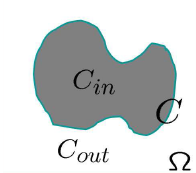
\includegraphics[scale=0.3]{./img/contour}\\
  \caption{Evolution of contour, courtesy of Bresson}\label{ACTE}
\end{figure}
In our case, ACM is used as a visual feature. The length of the maximum
length contour, number of points in the contour matrix and  number of rings are used as a feature.
\begin{figure}\centering
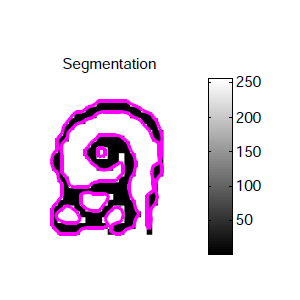
\includegraphics[scale=0.5]{./img/acm_crop}
  \caption{Segmentation using ACM}\label{LSM}
\end{figure}



\section{Random Projection}
Random Projection is a common dimensionality reduction technique\cite{shi}. The classes are classified based on L2-norm. We compare this technique with SVMTC. We also use RPT technique as feature for SVMTC. It is similar to PCA. The main difference is the introduction of random matrix.
\section{Character geometry}
Character geometry can serve as handy visual feature\cite{dileep}.
       \begin{itemize}
\item Euler Number - It is defined as the difference of number of objects and number of holes in a image.
 \item Regional area - It is defined as the ratio of the number of
the pixels in the skeleton to the total number of pixels in the image.
 \item Eccentricity - It is defined as the eccentricity of the
smallest ellipse that fits the skeleton of the image.
 \item Zonal Feature - It is a feature based on the directional rules.
        \end{itemize}
\section{Hu's Moments}
Image moment is a weighted average of pixel intensities. Properties that are derived from image moments include area and centroid. Information about image orientation can be obtained 
by taking second order moments. Scale invariant moments $\eta_{ij}$ are obtained by dividing properly scaled
$\mu_{00}$th moment as follows.
\begin{equation}
\eta_{ij} = \frac{\mu_{ij}}{{\mu_{00}}^{(1+\frac{i+j}{2})}}
\end{equation}
where i + j $\ge$ 2.
The $(p+q)$th order of moment is geometric moment $M_{pq}$ of a gray-level image is defined as
\begin{equation}
M_{pq} = \int_{-\infty}^\infty\int_{-\infty}^\infty x^py^pf(x,y)dxdy\\
\end{equation}
In the case of a digital image, the double integral of the above equation must be replaced by a summation\cite{flusser1}.\\
\begin{equation}
m_{pq}=\sum_{i=1}^n\sum_{j=1}^ni^pj^qf_{ij}\\
\end{equation}
where N is the size of the image and $f_{ij}$ are the grey levels of individual pixels.

\section{Affine moment invariants}
Affine moment invariants are image moments which is immune to affine transformation of image like
scaling, translation and rotation. In this case, we use Hu's set of invariant moments\cite{flusser2}.

\section{Gabor Filter}
The 2D-Gabor filter can serve as a statistical feature. It uses Gaussian kernel function.
We create a vector of this function values with 
different frequencies and orientation.The standard deviation and mean of this vector serves as a 
feature.
  \begin{equation}
f(x,y,\omega,\theta,\sigma_x,\sigma_y) = \frac{1}{2\pi\sigma_x\sigma_y}e^
{[\frac{-1}{2}((\frac{x}{\sigma_x})^2+(\frac{y}{\sigma_y})^2) + j\omega(xcos\theta +ysin\theta)]}
  \end{equation}
\section{Implementation}
The feature extraction is carried out by roger.m. We extracted  seven features based on Hu's Moments.
Hundred based on RPT. Three based on ACM. Three  hundred based on 2-D Gabor filter and the rest based on moment's invariants and character geometry.